%! TeX program = lualatex

\documentclass[11pt]{extarticle}

% Set 1-inch margins
\usepackage[margin=1in]{geometry}

% Set Times New Roman for text and Cambria Math for math fonts
\usepackage{fontspec}
\setmainfont{Times New Roman}

% Use Symbol font for non-alphabetic characters
\usepackage{textcomp}

% Set line spacing to single (no less than single-spacing)
\usepackage{setspace}
\setstretch{1.0}

% Package for handling citations
\usepackage[backend=biber,style=numeric,sorting=none]{biblatex}
\addbibresource{references.bib}

% For inserting images and subcaptions
\usepackage{graphicx,subcaption} 
\usepackage{svg}

% Begin document
\begin{document}

% TODO: Wordsmith "knowledge products" a bit more
% TODO: Review first sentence again
\textbf{Hypothesis:} Knowledge discovery is a fundamental procedure across disciplines but is time intensive and laborious.
\textbf{Framing knowledge discovery in category theoretic terminology would enable the furthered understanding of relationships between knowledge products.}

\textbf{Introduction:} Compositionality, the characteristic that ``describes and quantifies how complex things can be assembled out of simple parts''[1], is a concept ubiquitous across mathematics but is seen acutely in the fundamentals of category theory.
Simply put, category theory studies the "relationships that exist between things" which gives one a vantage point to think not on the minutiae of a particular problem but more broadly about how things in a problem space may ``fit together'' (i.e. ``composed together'').
This way of framing problems is beginning to permeate specific domains such as engineering system design [2], database architecture [3], and machine learning [4]. 

% TODO: Review the last sentence here -- could be said better and maybe allude to stronger tooling here
With this perspective in mind, a task common to nearly all disciplines is scrutinizing available data to generate novel insight about a particular topic or field -- a procedure more commonly referred to as ``knowledge discovery''.
Motivating this discussion is that knowledge discovery can appear similar across disciplines but due to domain specifics, adapting old discovery methods to novel applications can be a laborious process. 
At best, this may lead to productivity losses in the US workforce [5] and at worst could lead to poorly managed disaster responses [6].
\textbf{A category theory-informed framing of the knowledge discovery process gives a strong perspective to better understand relationships between knowledge products and how they may be most effectively composed together.}

% TODO: Include Objectives within this section
% TODO: Somehow call out the specific methods
\textbf{Research Plan:} I will dedicate my PhD studies at Harvard University to investigate the promise of applying category theory in knowledge discovery under the advisement of Professor Nathaniel Osgood.
There, I will pursue the following objectives:

\textbf{Objective 1: Map the Knowledge Discovery Process To Category Theoretic Language.}

To drive exploration of the general knowledge discovery process, I will pick three heterogeneous data sets that vary by how they are sampled over time and by what kind of data they contain. 
Then, I will construct general knowledge discovery pipelines to scrutinize these data sets through various data science techniques (such as clustering or prediction methods) to simulate deriving novel insights data in general.
After creating these pipelines, I will then explore manually how these data sets could be related to one another.

Once several relationships that could exist within and between data sets have been enumerated, I will then proceed to map these knowledge discovery processes on to various categorical structures.
First, I will use $\mathscr{C}$-sets, which describes a functor mapping a schema category $\mathscr{C}$ into the category $\mathbb{Set}$ (as objects) and functions between them (as morphisms) [@osgood] % TODO: Add a sentence after this about what this is exactly
Then, is the decorated copresheaf (known as "acsets") which is very helpful in relating these species of data and computing upon them [@lynch]

\textbf{Objective 2: Prototype Knowledge Discovery for a Specific Topic Using Category Theoretic Framing.}


To carry out this effort, I will use three strongly hetergeneous data sets to develop a study. 
The data I will use comprises of the following: [IPUMS](http://ipums.org/) census microdata for a variety of different demographic information across the globe and a ton for the USA, [ERA5](https://cds.climate.copernicus.eu/cdsapp#!/dataset/reanalysis-era5-single-levels?tab=overview) & [National Centers for Environmental Information](https://www.ncei.noaa.gov) These two datasets have such a wide array of climate related data for the entire globe on a fantastic time resolution, and [Pharmetrics Plus](https://www.iqvia.com/locations/united-states/library/fact-sheets/iqvia-pharmetrics-plus) a 35+ million USA patient database of patient medical records from across the entire country.
What motivates this particular selection of data sets is the significant differences between them: the IPUMS data is regularly sampled across the US at a state or coarse population level at regular and monthly time intervals, the ERA5 and NCEI data is also regularly sampled but at a much more granular time and temporal resolution, and the patient data set varies significantly by geospatial region as well as having extremely irregular or even random sampling intervals for patient encounters.

\textbf{Objective 3: Assess and Validate Insights from Category-Theory Informed Knowledge Discovery Prototype.}

\textbf{Objective 4: Explore Composing of Knowledge Discovery Processes.}

In the second year, after I have more adequately described and understood this study in terms of category theory, I will further explore how to meaningfully relate scientific studies together.
Inspired by thoughts from @bgavran's papers in applying Category Theory to Machine Learning (namely [Category Theory in Machine Learning](https://arxiv.org/abs/2106.07032) and [Position: Categorical Deep Learning is an Algebraic Theory of All Architectures](https://arxiv.org/abs/2402.15332)) 
**Interface a ACSet study configuration with Machine Learning tools.** As the current ACSet machinery is within Julia, we'll make liberal use of the [Tables.jl interface](https://github.com/JuliaData/Tables.jl) as probably the core interchange format.
**Interpret a statistic on top of the ACSet-based study.** This will be the crux of the study as to what is possible and what can be done within this framing. At this point will be some uncharted territory so will base again upon *An Algebraic Framework for Structured Epidemic Modeling*. Perhaps I will reach out to Simon Frost or @ndo885 at this stage as well.

\begin{figure}[!h]
 \begin{subfigure}{0.4\textwidth}
     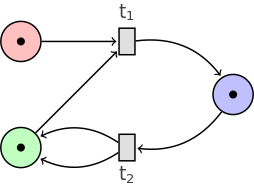
\includegraphics[width=\textwidth]{marking_1}
     \caption{\dots}
     \label{fig:a}
 \end{subfigure}
 \hfill
 \begin{subfigure}{0.4\textwidth}
     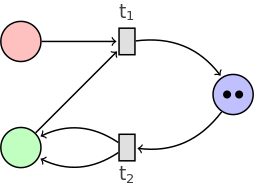
\includegraphics[width=\textwidth]{marking_2}
     \caption{\dots}
     \label{fig:b}
 \end{subfigure}
 
 \medskip
 \begin{subfigure}{0.4\textwidth}
     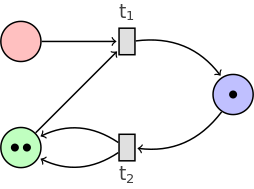
\includegraphics[width=\textwidth]{marking_3}
     \caption{\dots}
     \label{fig:c}
 \end{subfigure}
 \hfill
 \begin{subfigure}{0.4\textwidth}
     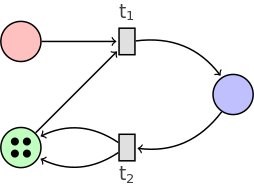
\includegraphics[width=\textwidth]{marking_4}
     \caption{\dots}
     \label{fig:d}
 \end{subfigure}

 \caption{Caption for all 4 figures}
 \label{Label}

\end{figure}

\textbf{Intellectual Merit:} This project aims to advance fundamental knowledge by applying category theory to the formalization of research studies as compositional objects. 
By introducing a mathematically rigorous framework to model and relate studies across diverse fields, the project addresses foundational challenges in engineering system design, database architecture, and data integration. 
The use of category theory to harmonize heterogeneous datasets—ranging from census microdata to climate and patient records—represents a transformative approach that could redefine how information sciences handle complex, multi-source data, offering new paradigms for knowledge synthesis and data interoperability.

\textbf{Broader Impacts:} This project introduces a new framework for formalizing research studies as compositional objects, which could revolutionize how large-scale, complex systems are analyzed across fields such as engineering, computer, and information sciences. By establishing a structured approach to integrating diverse methodologies and datasets, this work has the potential to enhance research reproducibility, scalability, and collaboration across disciplines. The compositional framework could enable the development of new computational tools and models that support more efficient, modular research designs, leading to broad applications in optimizing workflows, improving data interoperability, and advancing the frontiers of scientific discovery in both theoretical and applied domains.

\textbf{References:} [1] \textit{Compositionality}, 2024. [2] \textit{ACT4ED}, MIT 1.S980 [3] \textit{Algebraic Databases}, Shultz, et. al., 2016. [4] \textit{Category theory in machine learning}, Gavranović, 2021. [5] \textit{Measuring the impact of knowledge loss: a longitudinal study} Massingham [6] \textit{Emergency Preparedness for Vulnerable Populations}, Nick


\end{document}
